The following sections presents an overview of the queue and query implementation of Savannah's server software.
\subsubsection{Queue}

As mentioned in \autoref{sect:ssArchAndDesign} Savannah is designed around a producer-consumer pattern centered on a FIFO queue, implemented in the \code{EventQueue} class.
The UML diagram in \autoref{figure:EventUML} shows the event queue implementation and closely related classes.
The event queue is a \code{LinkedList<Event>} object instantiated as a \code{Queue<Event>}, this instantiation defaults to a FIFO queue through
the \code{queue.add(event)} and \code{queue.remove()} methods. \code{EventQueue} is implemented as a singleton to ensure that Savannah never has access to more than one queue.
Events are implemented through the \code{Event} interface that \code{RequestEvent} and \code{CommitEvent} implements.
Finally the \code{EventHandler} class is responsible for removing events from the queue and make sure they are processed by the server. It is started as a thread and
continuously probes the queue for content. All queue access is synchronized, through the use of the Java \code{synchronized} keyword, to avoid race conditions.

\begin{figure}[H]
 \centering
  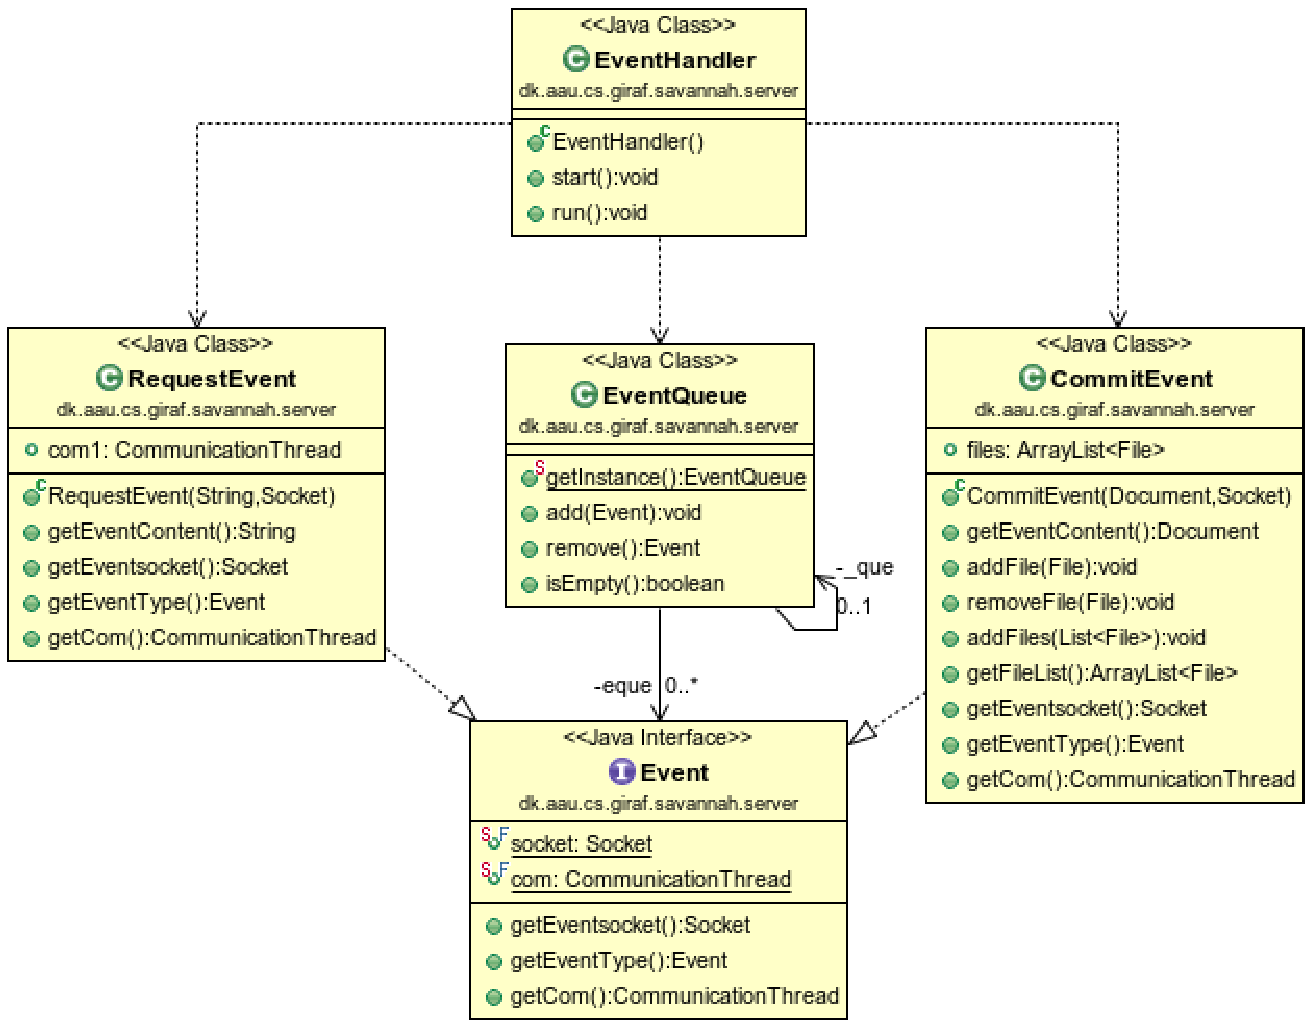
\includegraphics[scale=0.65]{images/EventQueue}
  \caption{EventQueue UML diagram.}
  \label{figure:EventUML}
\end{figure}

An event contains a reference to the socket on which the connection was made and the event content, which is either an XML document or a \code{String} containing certificates
needed to query profiles from the database.

\subsubsection{Query creation and handling}

The UML diagram in \autoref{figure:queryUML} shows the \code{EventHandler} and related classes for building SQL queries, querying the database, and building XML documents.
The \code{Eventhandler} instantiates a \code{RequestHandler} and a \code{CommitHandler}, which are responsible for handling request- or commit events.
Each of the handlers instatiate a \code{QueryBuilder} and a \code{QueryHandler}. The \code{QueryBuilder} creates SQL queries based on the event content. The queries are forwarded to the \code{QueryHandler}
that interacts with the database and, if the event is a \code{RequestEvent}, returns a \code{ResultSet} object. Finally the \code{Resultset} object is forwarded to the \code{XMLBuilder} that builds an sw6ml document,
in \code{String} form, that can be returned to the requesting party. 
\begin{figure}[H]
 \centering
  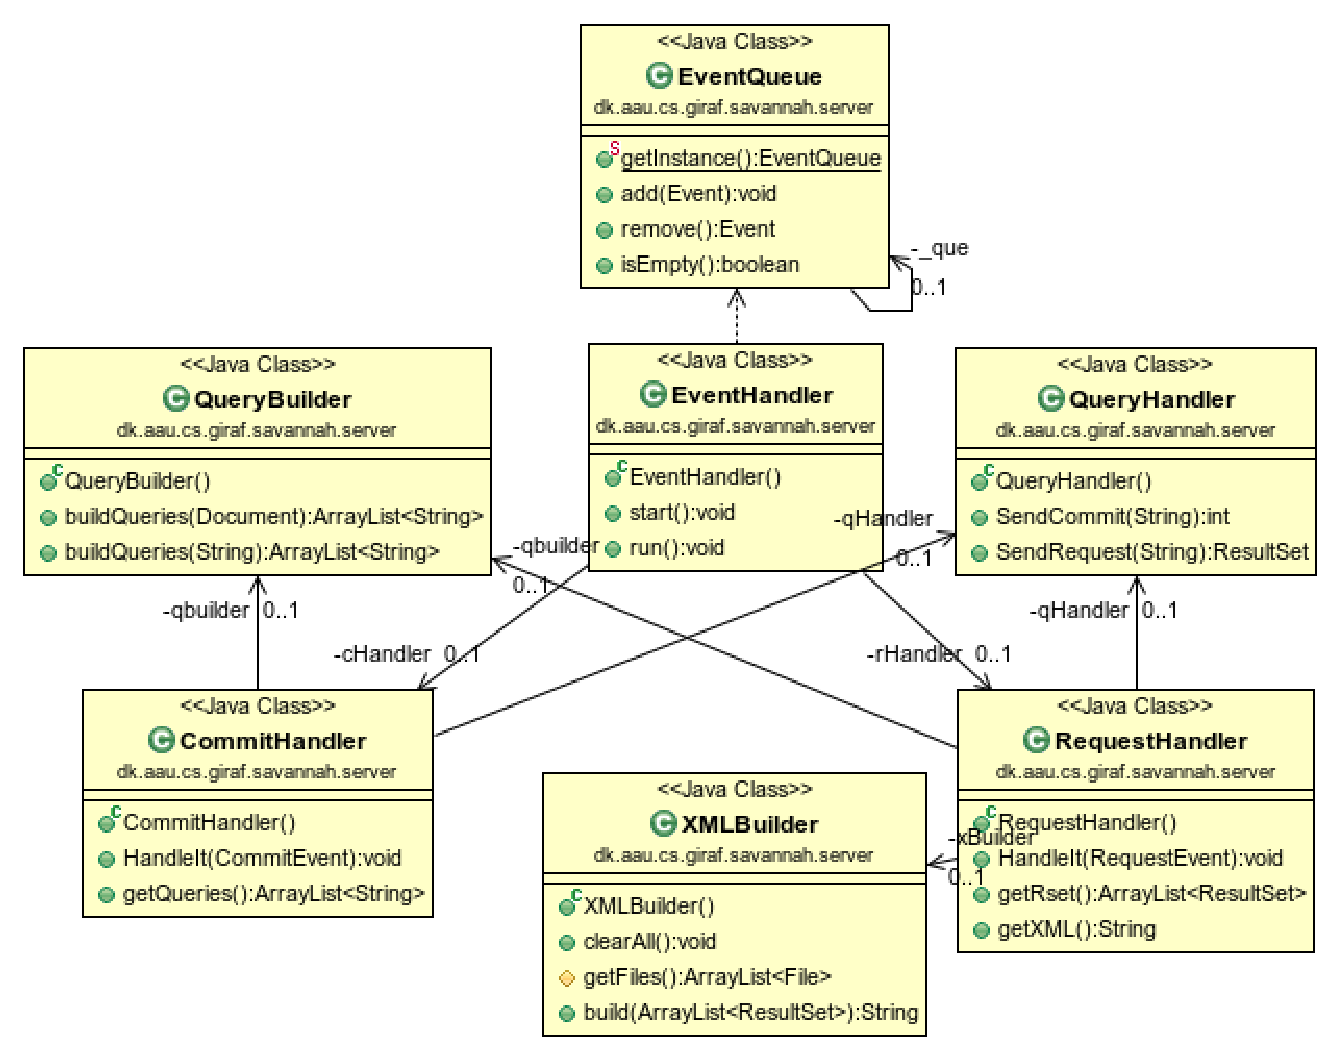
\includegraphics[scale=0.65]{images/queryhandling}
  \caption{Query handling UML diagram.}
  \label{figure:queryUML}
\end{figure}

